
\appendix

\section{Applicability Boundary: Stochastic VLA Diversity}
\label{sec:applicability}

\looseness=-1 The multi-sample pipeline requires stochastic action diversity across samples. We validate this prerequisite on two VLA architectures: SmolVLA~\cite{shukor2025smolvla} (flow matching, 0.4B) and OpenVLA-OFT~\cite{kim2024openvla} (deterministic $L_1$ regression, 7B).

SmolVLA produces meaningfully diverse action samples across all dimensions via its flow-matching generative process. In contrast, OpenVLA-OFT's deterministic $L_1$ regression produces near-identical outputs: mean pairwise $L_2{=}0.00436$ across $K{=}2$ samples, with $97.3$\% of steps below $0.01$. The uncertainty gate never fires, and multi-sample selection is vacuous.

This result establishes an architectural boundary: multi-sample inference-time correction is specific to stochastic generative VLAs (flow matching, diffusion). Deterministic VLAs lack the action diversity that selection and correction rely on. The boundary is architectural, not a limitation of our method: any inference-time approach that draws multiple action candidates requires the base policy to produce diverse samples.

\section{Cross-VLA Analysis: Model Capability Dependency}
\label{sec:cross_vla}

\looseness=-1 We evaluate the CRM degradation pattern on $\pi_{0.5}$~\cite{black2025pi05} (3.6B, flow matching), where near-saturated baselines reach 94--98\% (Table~\ref{tab:pi05}). The same K-matched design ($K{=}2$, $\varepsilon{=}0.2$, shared CRM architecture) is used. Unconditional CRM correction degrades all four suites: Long suffers $-$17.0\,pp ($94.0{\to}77.0$\%, the largest single-suite drop across both VLAs), Goal $-$14.0\,pp, Object $-$6.0\,pp, and Spatial $-$2.0\,pp. Multi-seed evaluation ($n{=}3$; Table~\ref{tab:pi05_multiseed}) confirms the pattern, with Long degradation reaching $-$17.5\,pp. As on SmolVLA, the CRM is trained on three suites and Long is out-of-distribution, amplifying the harm. The degradation on all four suites of both VLAs is consistent with the core thesis: when most steps are already near-optimal, learned correction noise has proportionally greater impact, and this pattern generalizes across model scale.

\begin{table}[h]
\centering
\caption{Cross-VLA degradation analysis: $\pi_{0.5}$ (3.6B) on LIBERO. Near-saturated baselines (94--98\%) are degraded by unconditional CRM correction on all four suites, with Long suffering $-$17.0\,pp (the largest single-seed drop across both VLAs).}
\label{tab:pi05}
\small
\begin{tabular}{lccc}
\toprule
Suite & VLA-only ($K{=}1$) & CRM always-on ($K{=}2$) & $\Delta_{\mathrm{CRM}}$ \\
\midrule
Spatial & $98.0$ & $96.0$ & $-2.0$ \\
Object & $96.5$ & $90.5$ & $-6.0$ \\
Goal & $95.5$ & $81.5$ & $-14.0$ \\
Long & $94.0$ & $77.0$ & $-17.0$ \\
\bottomrule
\addlinespace[2pt]
\multicolumn{4}{l}{\scriptsize $n{=}1$ seed; $\varepsilon{=}0.2$, same CRM architecture as SmolVLA.}\\
\multicolumn{4}{l}{\scriptsize VLA-only and CRM always-on evaluated on different servers (seed-matched); cross-server}\\
\multicolumn{4}{l}{\scriptsize variance is ${\leq}$4\,pp on short suites, and all degradation directions are consistent.}
\end{tabular}
\end{table}


\section{Threshold Sensitivity Analysis}
\label{sec:tau_sweep}

\begin{figure}[h]
  \centering
  \begin{minipage}[t]{0.48\linewidth}
    \centering
    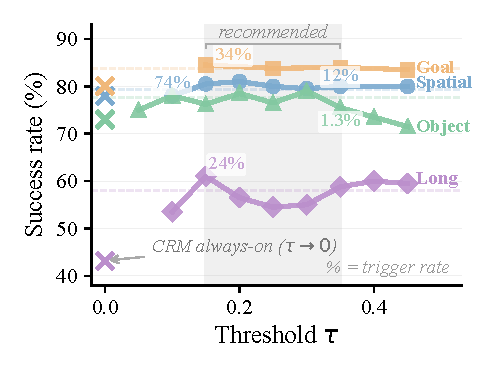
\includegraphics[width=\linewidth]{fig_tau_sweep.pdf}\\[-2pt]
    {\small (a)}
  \end{minipage}
  \hfill
  \begin{minipage}[t]{0.48\linewidth}
    \centering
    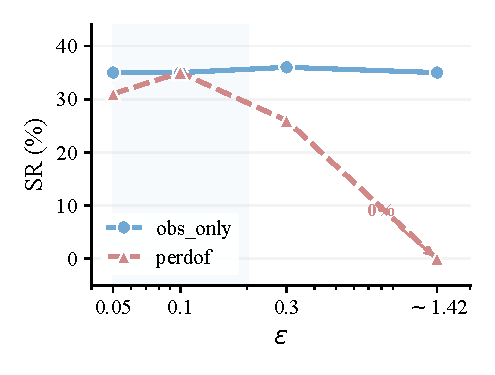
\includegraphics[width=\linewidth]{magnitude_curve.pdf}\\[-2pt]
    {\small (b)}
  \end{minipage}
  \caption{(a)~Threshold sensitivity on SmolVLA. Solid: CRM $\tau$-gated SR; dashed: VLA-only baselines; $\times$: CRM always-on. SR varies by ${\leq}$2\,pp over a $3{\times}$ range of $\tau$. (b)~Correction magnitude sensitivity on Spatial (seed 42): observation-only CRM (blue) is robust across $\varepsilon \in [0.05, 0.2]$; per-DOF variant (red) collapses at high $\varepsilon$.}
  \label{fig:tau_sweep}
\end{figure}

\begin{table}[h]
\centering
\caption{SmolVLA threshold sensitivity ($\varepsilon{=}0.2$), complete $\tau$-sweep across all four LIBERO suites. $\tau$ primarily controls intervention frequency: on Spatial ($\tau{=}0.15$--$0.45$), trigger rate changes $5.5{\times}$ while SR varies by ${\leq}$2\,pp. Long is out-of-distribution (OOD) for the CRM (Section~\ref{sec:exp_setup}).}
\label{tab:tau_sweep}
\small
\begin{tabular}{llccc}
\toprule
Suite & $\tau$ & SR (\%) & Trigger (\%) & $n$ \\
\midrule
Spatial & 0.10 & 78.0 & 74.4 & 1 \\
Spatial & 0.15 & 80.5 & 40.7 & 1 \\
Spatial & 0.20 & 81.0 & 26.7 & 1 \\
Spatial & 0.25 & 80.0 & 19.5 & 3 \\
Spatial & 0.30 & 79.5 & 16.8 & 1 \\
Spatial & 0.35 & 80.0 & 12.2 & 1 \\
Spatial & 0.45 & 80.0 & 7.3 & 1 \\
\midrule
Goal & 0.15 & 84.5 & 34.4 & 2 \\
Goal & 0.25 & 83.8 & 8.1 & 3 \\
Goal & 0.35 & 84.0 & 2.3 & 2 \\
Goal & 0.45 & 83.5 & 0.9 & 1 \\
\midrule
Object & 0.05 & 75.0 & --- & 1 \\
Object & 0.10 & 78.0 & --- & 1 \\
Object & 0.15 & 76.2 & 16.6 & 3 \\
Object & 0.20 & 78.5 & --- & 1 \\
Object & 0.25 & 76.5 & 3.5 & 2 \\
Object & 0.30 & 79.0 & 2.3 & 1 \\
Object & 0.35 & 75.5 & 1.3 & 1 \\
Object & 0.40 & 73.5 & 0.9 & 1 \\
Object & 0.45 & 71.5 & 0.8 & 1 \\
\midrule
Long$^{\dagger}$ & 0.10 & 53.5 & 61.3 & 1 \\
Long$^{\dagger}$ & 0.15 & 61.0 & 23.8 & 2 \\
Long$^{\dagger}$ & 0.20 & 56.5 & 8.9 & 2 \\
Long$^{\dagger}$ & 0.25 & 54.5 & 4.4 & 2 \\
Long$^{\dagger}$ & 0.30 & 55.0 & --- & 2 \\
Long$^{\dagger}$ & 0.35 & 58.8 & 1.2 & 2 \\
Long$^{\dagger}$ & 0.40 & 60.0 & 0.4 & 1 \\
Long$^{\dagger}$ & 0.45 & 59.5 & 0.3 & 1 \\
\bottomrule
\addlinespace[2pt]
\multicolumn{5}{l}{\scriptsize $n$: seeds averaged. ${}^{\dagger}$CRM is OOD on Long (trained on 3 suites).}\\
\multicolumn{5}{l}{\scriptsize ---: trigger rate not recorded for this run.}
\end{tabular}
\end{table}

\begin{table}[h]
\centering
\caption{$\pi_{0.5}$ threshold sensitivity ($\varepsilon{=}0.2$). The plateau pattern holds on the three evaluated suites (Spatial, Goal, Long): trigger rate varies substantially with $\tau$, but SR changes remain small. Extended $\tau$ range on Goal ($0.15$--$0.90$) suggests robustness.}
\label{tab:tau_sweep_pi05}
\small
\begin{tabular}{llccc}
\toprule
Suite & $\tau$ & SR (\%) & Trigger (\%) & $n$ \\
\midrule
Spatial & 0.15 & 97.0 & 11.2 & 1 \\
Spatial & 0.25 & 96.8 & 4.4 & 2 \\
Spatial & 0.35 & 96.5 & 2.6 & 1 \\
\midrule
Goal & 0.15 & 92.0 & 17.4 & 1 \\
Goal & 0.25 & 87.5 & 9.1 & 3 \\
Goal & 0.35 & 87.5 & 5.7 & 1 \\
Goal & 0.50 & 87.0 & 2.1 & 1 \\
Goal & 0.70 & 87.0 & 1.0 & 1 \\
Goal & 0.90 & 89.0 & 0.4 & 1 \\
\midrule
Long & 0.15 & 84.0 & 11.4 & 1 \\
Long & 0.25 & 81.0 & 4.4 & 3 \\
Long & 0.35 & 81.0 & 2.4 & 1 \\
\bottomrule
\end{tabular}
\end{table}

\looseness=-1 Tables~\ref{tab:tau_sweep} and~\ref{tab:tau_sweep_pi05} report success rates as a function of the uncertainty threshold $\tau$ on SmolVLA and $\pi_{0.5}$, respectively. On both models, $\tau$ primarily controls intervention frequency rather than final SR: on SmolVLA Spatial, trigger rate drops from 40.7\% ($\tau{=}0.15$) to 7.3\% ($\tau{=}0.45$), a $5.5{\times}$ reduction, while SR varies by only 1.5\,pp (79.5--81.0\%). On $\pi_{0.5}$ Spatial, a similar pattern holds (11.2\%$\to$2.6\% trigger, 0.5\,pp SR range). This plateau effect indicates that the CRM needs to intervene on only a small fraction of steps to reach its performance ceiling.

\looseness=-1 The Long suite, where the CRM is OOD, exhibits wider SR variation across $\tau$: from 53.5\% ($\tau{=}0.10$, trigger 61.3\%) to 61.0\% ($\tau{=}0.15$, trigger 23.8\%). Notably, $\tau{=}0.15$ exceeds VLA-only (58.0\%) by 3\,pp, while the shared threshold $\tau{=}0.25$ yields 54.5\%. This suite-dependence of optimal $\tau$ motivates adaptive threshold selection as future work (Section~\ref{sec:limitations}). On $\pi_{0.5}$ Goal, extending $\tau$ from 0.15 to 0.90 confirms the plateau: SR remains within 87.0--92.0\% as trigger rate drops from 17.4\% to 0.4\%.

\looseness=-1 Goal shows a stable plateau (${\sim}$1\,pp variation, 83.5--84.5\%) across $\tau$, within per-seed noise (Table~\ref{tab:main}, std ${\sim}$1--2\,pp). Object exhibits wider variation: SR ranges from 71.5\% ($\tau{=}0.45$) to 79.0\% ($\tau{=}0.30$), a 7.5\,pp spread. At high $\tau$ (${\geq}0.35$), Object SR degrades because the gate rarely fires (${\leq}$1.3\%) and $K{=}2$ argmin alone underperforms VLA-only on this suite. The within-suite relationship between trigger rate and SR is not monotonic, consistent with the CRM providing limited correction quality on steps where the VLA's errors are systematic rather than stochastic. The cross-suite positive correlation (higher trigger rate correlating with larger improvement, Figure~\ref{fig:trigger_scatter}) remains the primary mechanism evidence.

\looseness=-1 \textbf{Note on $\varepsilon$.}\enspace Both CRM always-on and CRM $\tau$-gated in Table~\ref{tab:main} use $\varepsilon{=}0.2$, matching the $\tau$-sweep configuration. The K-matched design ensures the only variable is calibrated gating ($\tau{\to}0$ vs.\ calibrated $\tau$).


\section{Uncertainty Proxy Comparison}
\label{sec:proxy_comparison}

\looseness=-1 Table~\ref{tab:proxy_comparison} (main text) compares four candidate uncertainty proxies against $K{=}10$ sample variance as ground truth. CRM correction magnitude (the $L_2$ norm of the CRM's predicted residual) is attractive because it requires no extra VLA forward passes, but correlates weakly with true uncertainty ($\rho < 0.16$): the CRM predicts similar-magnitude corrections regardless of whether the VLA is confident or uncertain. FMVD, which measures dispersion in the flow-matching velocity field, performs worse still ($\rho{=}0.083$). The $K{=}2$ pairwise $L_2$ distance achieves near-perfect correlation ($\rho{=}0.9979$) at the cost of one additional VLA forward pass, which is absorbed by batched inference (Section~\ref{sec:efficiency}).


\section{Reproducibility Details}
\label{sec:reproducibility}

\paragraph{Hardware.}
All experiments run on NVIDIA RTX 4090 GPUs (24\,GB VRAM). SmolVLA inference uses a single GPU; CRM training and evaluation each use a single GPU.

\paragraph{CRM training.}
The CRM is trained on three suites (Spatial, Object, Goal; 30 tasks, ${\sim}$88K samples) for 50 epochs with Adam ($\mathrm{lr}{=}10^{-3}$, batch size 32) in ${\sim}$6 GPU-hours on 1$\times$ RTX 4090. Long is excluded from CRM training; Long-suite evaluation tests cross-suite generalization. Precomputing the $K{=}10$ forward-pass cache (required once per suite) takes ${\sim}$2 GPU-hours per suite.

\paragraph{Evaluation.}
Each suite evaluation (20 rollouts $\times$ 10 tasks $\times$ 300 max steps) takes ${\sim}$2.5 GPU-hours. A full 5-method $\times$ 4-suite $\times$ 3-seed experiment requires ${\sim}$150 GPU-hours total.

\paragraph{Software.}
PyTorch 2.4, Transformers 4.45, LIBERO (MuJoCo-based). Code and CRM checkpoints will be released upon acceptance.


\section{Computational Efficiency}
\label{sec:efficiency}

Table~\ref{tab:efficiency} (main text) compares the computational cost of each method. The key insight is that batched inference absorbs the cost of the second VLA forward pass: $K{=}2$ latency matches $K{=}1$ because both samples share the same prefix encoding and flow-matching denoising runs in parallel.


\section{Extended 8-Seed Analysis on Spatial}
\label{sec:8seed}

\begin{table}[h]
\centering
\caption{Per-seed success rates (\%) on LIBERO-Spatial for VLA-only vs.\ CRM $\tau$-gated ($K{=}2$, $\tau{=}0.25$). All 8 seeds use identical $K{=}2$ configuration (code-verified).}
\label{tab:8seed}
\small
\begin{tabular}{lccc}
\toprule
Seed & VLA-only & CRM $\tau$-gated & $\Delta$ \\
\midrule
42 & 80.0 & 82.0 & $+2.0$ \\
43 & 79.0 & 80.0 & $+1.0$ \\
44 & 78.5 & 80.5 & $+2.0$ \\
45 & 80.0 & 80.0 & $+0.0$ \\
46 & 80.5 & 80.0 & $-0.5$ \\
47 & 80.0 & 81.5 & $+1.5$ \\
48 & 79.5 & 81.0 & $+1.5$ \\
49 & 78.5 & 82.0 & $+3.5$ \\
\midrule
Mean$\pm$std & $79.5 \pm 0.8$ & $80.9 \pm 0.9$ & $+1.4$ \\
\bottomrule
\end{tabular}
\end{table}

\looseness=-1 Table~\ref{tab:8seed} reports per-seed results for the extended 8-seed paired analysis on LIBERO-Spatial. A paired $t$-test yields $\Delta{=}{+}1.4$\,pp, $p{=}0.017$ ($n{=}8$), reaching statistical significance at $\alpha{=}0.05$. Six of eight seeds show positive $\Delta$; the two non-positive seeds ($\Delta{=}0.0$ and $\Delta{=}{-}0.5$) are consistent with measurement noise rather than systematic degradation. This analysis provides the strongest statistical evidence that calibrated $\tau$-gating produces a genuine improvement on the suite where the uncertainty gate fires most frequently (trigger rate ${\sim}$20\%).


\section{Additional Ablations}
\label{sec:additional_ablations}

\begin{table}[h]
\centering
\caption{Supplementary ablations on SmolVLA. $K{=}10$ argmin~\cite{chen2026reconvla}: argmin-to-centroid selection over 10 samples, no learned correction. $K{=}2$ mean: centroid of two samples, no CRM. Neither consistently improves over VLA-only.}
\label{tab:ablations}
\small
\begin{tabular}{lcccccc}
\toprule
Method & $K$ & Spatial (\%) & Object (\%) & Goal (\%) & Long (\%) \\
\midrule
VLA-only & 1 & $79.3 \pm 0.8$ & $77.7 \pm 1.3$ & $83.7 \pm 1.3$ & $58.0 \pm 1.5$ \\
$K{=}10$ argmin & 10 & $80.3 \pm 1.0$ & $77.3 \pm 1.5$ & $80.8 \pm 0.3$ & $56.5^{\dagger}$ \\
$K{=}2$ mean & 2 & --- & $77.5 \pm 2.3$ & $83.0 \pm 2.2$ & $57.0^{\dagger}$ \\
\bottomrule
\addlinespace[2pt]
\multicolumn{6}{l}{\scriptsize $n{=}3$ seeds unless noted; ${}^{\dagger}n{=}1$; --- = omitted (computational budget).}
\end{tabular}
\end{table}

\looseness=-1 Table~\ref{tab:ablations} reports two ablations that isolate multi-sample selection without learned correction. $K{=}10$ argmin invests $10{\times}$ the VLA forward passes but hurts on Goal ($-$2.9\,pp) and Long ($-$1.5\,pp): selection alone cannot fix systematic errors. $K{=}2$ mean offers no learned correction mechanism ($-$0.7\,pp Goal, $-$1.0\,pp Long; Long is single-seed preliminary), confirming that multi-sampling alone is insufficient.


\section{CRM Always-On Per-Seed Analysis}
\label{sec:crm_perseed}

\begin{table}[h]
\centering
\caption{Per-seed success rates (\%) for CRM always-on ($K{=}2$, $\varepsilon{=}0.2$, $\tau{\to}0$). SmolVLA uses seeds 42--46 ($n{=}5$); Table~\ref{tab:main} reports $n{=}3$ means from seeds 42--44. $\pi_{0.5}$ rows show fewer seeds; full multi-seed results in Table~\ref{tab:pi05_multiseed}.}
\label{tab:crm_perseed}
\small
\begin{tabular}{llccccccc}
\toprule
Model & Suite & s42 & s43 & s44 & s45 & s46 & $n$ & Mean$\pm$Std \\
\midrule
SmolVLA & Spatial & 79.0 & 76.0 & 79.0 & 77.0 & 78.5 & 5 & $77.9 \pm 1.3$ \\
SmolVLA & Object & 71.0 & 73.5 & 74.5 & 74.5 & 67.5 & 5 & $72.2 \pm 3.0$ \\
SmolVLA & Goal & 80.0 & 79.5 & 80.5 & 82.0 & 80.0 & 5 & $80.4 \pm 1.0$ \\
SmolVLA & Long & 41.0 & 45.5 & 43.0 & --- & --- & 3 & $43.2 \pm 2.3$ \\
\midrule
$\pi_{0.5}$ & Spatial & 96.0 & --- & --- & --- & --- & 1 & $96.0$ \\
$\pi_{0.5}$ & Object & 90.5 & 92.0 & --- & --- & --- & 2 & $91.2 \pm 1.1$ \\
$\pi_{0.5}$ & Goal & 81.5 & --- & --- & --- & --- & 1 & $81.5$ \\
$\pi_{0.5}$ & Long & 77.0 & --- & --- & --- & --- & 1 & $77.0$ \\
\bottomrule
\addlinespace[2pt]
\multicolumn{9}{l}{\scriptsize ---: not evaluated. SmolVLA Long s45 incomplete (excluded).}
\end{tabular}
\end{table}

\looseness=-1 Table~\ref{tab:crm_perseed} reports per-seed CRM always-on results. SmolVLA means over seeds 42--44 match Table~\ref{tab:main}; the extended 5-seed means show consistent degradation patterns across all suites. Object exhibits the highest per-seed variance (std${=}$3.0), driven by seed 46 (67.5\%), suggesting interaction between CRM noise injection and task-specific stochasticity.


\section{\texorpdfstring{$\pi_{0.5}$}{Pi-0.5} Extended Multi-Seed Results}
\label{sec:pi05_multiseed}

\begin{table}[h]
\centering
\caption{$\pi_{0.5}$ (3.6B) per-seed success rates (\%) across three methods and four LIBERO suites from dedicated multi-seed evaluation runs. Table~\ref{tab:pi05} reports seed-42 matched pairs from separate runs; per-seed differences (${\leq}$4\,pp) reflect cross-server variance and evaluation stochasticity.}
\label{tab:pi05_multiseed}
\small
\begin{tabular}{llccccc}
\toprule
Suite & Method & s42 & s43 & s44 & $n$ & Mean$\pm$Std \\
\midrule
Spatial & VLA-only & 98.0 & 97.5 & 98.5 & 3 & $98.0 \pm 0.5$ \\
Spatial & CRM always-on & 96.5 & 97.0 & 97.0 & 3 & $96.8 \pm 0.3$ \\
Spatial & CRM $\tau$-gated & 96.5 & 98.0 & 97.0 & 3 & $97.2 \pm 0.8$ \\
\midrule
Object & VLA-only & 100.0 & 98.5 & 99.5 & 3 & $99.3 \pm 0.8$ \\
Object & CRM always-on & 89.0 & 87.0 & 88.0 & 3 & $88.0 \pm 1.0$ \\
Object & CRM $\tau$-gated & 85.5 & 85.0 & 88.0 & 3 & $86.2 \pm 1.6$ \\
\midrule
Goal & VLA-only & 98.0 & 97.0 & 97.5 & 3 & $97.5 \pm 0.5$ \\
Goal & CRM always-on & 85.5 & 83.0 & 85.0 & 3 & $84.5 \pm 1.3$ \\
Goal & CRM $\tau$-gated & 89.5 & 89.5 & 86.5 & 3 & $88.5 \pm 1.7$ \\
\midrule
Long & VLA-only & 94.0 & 95.5 & 95.5 & 3 & $95.0 \pm 0.9$ \\
Long & CRM always-on & 77.0 & 79.5 & 76.0 & 3 & $77.5 \pm 1.8$ \\
Long & CRM $\tau$-gated & 80.5 & 80.5 & 83.0 & 3 & $81.3 \pm 1.4$ \\
\bottomrule
\addlinespace[2pt]
\multicolumn{7}{l}{\scriptsize VLA-only and CRM evaluated on different servers (seed-matched).}
\end{tabular}
\end{table}

\looseness=-1 Table~\ref{tab:pi05_multiseed} extends the single-seed results in Table~\ref{tab:pi05} to $n{=}3$ seeds per condition on $\pi_{0.5}$. Unconditional CRM correction degrades all four suites relative to VLA-only, confirming the single-seed pattern with $n{=}3$: Long suffers $-$17.5\,pp ($95.0{\to}77.5$), the largest single-suite degradation across both VLAs. On Object, CRM $\tau$-gated ($86.2$\%) performs below CRM always-on ($88.0$\%), indicating that gating recovery depends on the quality of the underlying CRM---which diminishes when the base policy is near-optimal (VLA-only $99.3$\%). On Long, $\tau$-gating recovers 3.8\,pp relative to CRM always-on ($81.3$ vs.\ $77.5$), consistent with OOD suppression. Goal $\tau$-gating ($88.5{\pm}1.7$) partially recovers the $-$13.0\,pp CRM degradation ($97.5{\to}84.5$).


\section{K-Sweep Analysis}
\label{sec:k_sweep}

\begin{table}[h]
\centering
\caption{Effect of sample count $K$ on CRM always-on performance (SmolVLA, LIBERO-Object, $\varepsilon{=}0.2$). Increasing $K$ beyond 2 provides marginal improvement; $K{=}10$ yields the highest SR but at $5{\times}$ the VLA cost.}
\label{tab:k_sweep}
\small
\begin{tabular}{lcccc}
\toprule
$K$ & VLA calls & Seeds & SR (Mean$\pm$Std) & $\Delta$ vs.\ $K{=}2$ \\
\midrule
2 & 2 & 5 & $72.2 \pm 3.0$ & --- \\
5 & 5 & 2 & $73.2 \pm 0.4$ & $+1.0$ \\
10 & 10 & 1 & $78.0$ & $+5.8$ \\
20 & 20 & 2 & $74.5 \pm 1.4$ & $+2.3$ \\
\bottomrule
\addlinespace[2pt]
\multicolumn{5}{l}{\scriptsize $K{=}2$: from Table~\ref{tab:crm_perseed} ($n{=}5$). $K{=}10$ uses $\varepsilon{=}0.05$ (single seed).}
\end{tabular}
\end{table}

\looseness=-1 Table~\ref{tab:k_sweep} varies the sample count $K$ for CRM always-on on LIBERO-Object. Performance is relatively stable across $K{=}2$--$20$ (72.2--78.0\%), with $K{=}10$ showing the highest point estimate but at $5{\times}$ the VLA forward-pass cost and with only a single seed. The marginal gain from larger $K$ does not justify the computational cost, supporting the paper's use of $K{=}2$ with calibrated gating as the preferred operating point.

\section{Negative Results: Alternative CRM Designs}
\label{sec:negative_results}

\looseness=-1 We summarize four design alternatives that were systematically evaluated and failed, providing guidance for future work.

\paragraph{Per-DOF uncertainty conditioning.}
Conditioning the CRM on per-degree-of-freedom uncertainty features (rather than observation-only) causes progressive collapse: with uncapped correction magnitude, SR drops to 0\% consistently across seeds; even at $\varepsilon{=}0.3$, SR recovers only to 4--6\% vs.\ 77\% for observation-only (17 experiments). Exposing per-DOF uncertainty amplifies dimension-correlated correction noise, suggesting that lower-dimensional conditioning is preferable for small CRMs.

\paragraph{Single-sample correction (K=1 CRM with ACCG).}
Bypassing multi-sampling entirely---using a single VLA forward pass with approximate conformal correction guidance (ACCG)---yields SR of 7--12\%, a catastrophic degradation from VLA-only (77.7\%; 8 experiments). Without diverse samples, the pairwise distance gate cannot fire and the CRM receives no useful uncertainty signal. Multi-sampling is a necessary enabler, not merely a convenience.

\paragraph{Leave-task-out generalization.}
When the CRM is evaluated on held-out tasks within the same suite (Object), SR drops to ${\sim}$2\% vs.\ ${\sim}$80\% VLA-only (2 experiments). The CRM is effectively task-set-specific: it memorizes correction patterns for seen tasks rather than learning generalizable residuals. This motivates future work on task-agnostic correction architectures.

\paragraph{Learned uncertainty head.}
Training a separate uncertainty prediction head to replace the $K{=}2$ pairwise distance probe yields SR of 11--14\% with near-zero trigger rates (3 experiments). The effective uncertainty signal arises from the flow-matching process's inherent stochasticity across forward passes, which cannot be captured by a deterministic learned predictor from a single pass.

\smallskip\noindent\textit{AI tools assisted with code and manuscript.}
